\chapter{Climate Analysis}
\label{chapter:climate}
\section{ECMWF Reanalysis v5 Dataset}

The ECMWF Reanalysis v5 (ERA5) dataset (\cite{era5}) was selected for correlating with tree genus classification due to its extensive and high-resolution climate data, which includes variables such as temperature, precipitation, and soil moisture. This dataset offers detailed historical weather information, capturing both spatial and temporal variations essential for understanding the environmental conditions that impact tree growth and distribution. By leveraging ERA5 data, this study aimed to explore how different climate factors might influence the abundance of various tree genera.

\begin{figure}[ht]
    \centering
    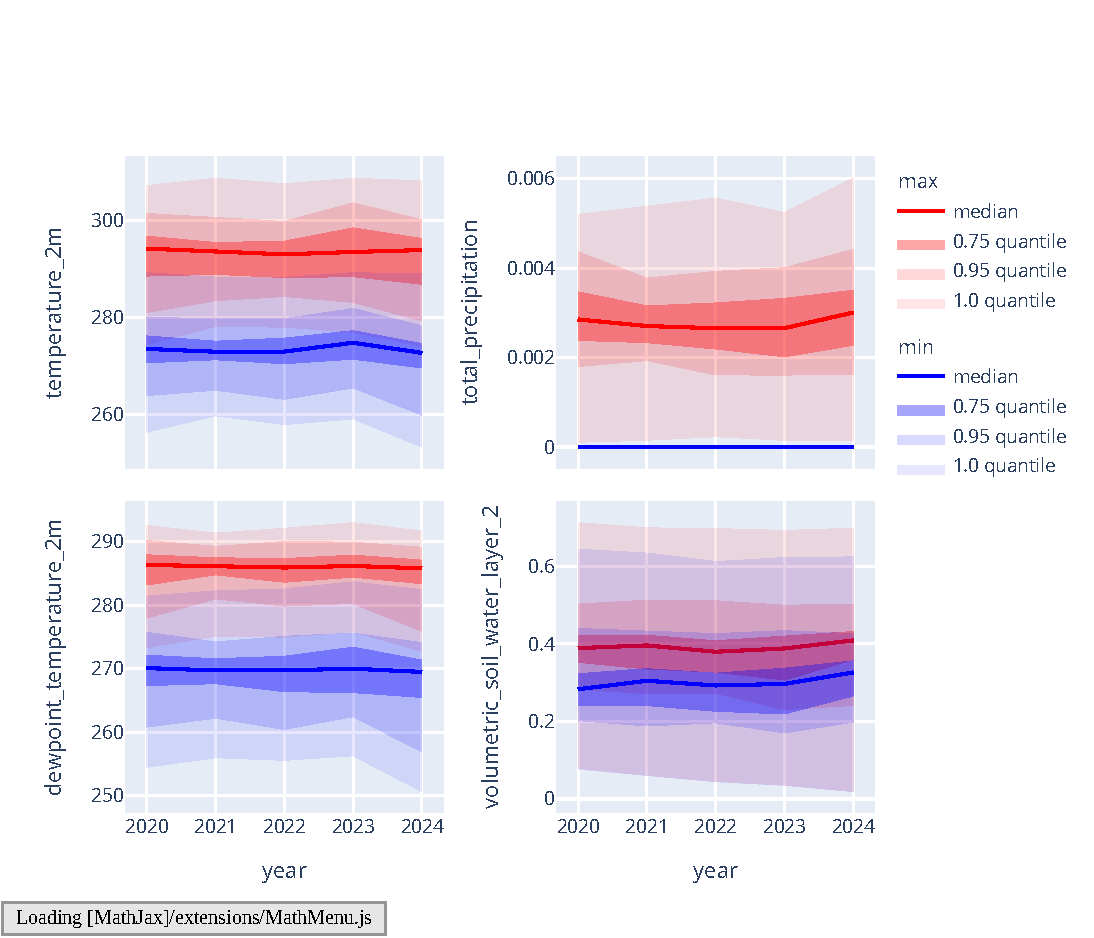
\includegraphics[width=0.9\linewidth, trim={20pt 20pt 10pt 40pt}, clip]{figures/figures_climate/selected_variables_stats.pdf}
    \caption{Median and quantiles of various monthly ERA5 variables by year. The data was downloaded from \cite{era5_dataset}, where detailed information is available.}
    \label{fig:selected_variables_stats}
\end{figure}

As the ERA5 dataset contains numerous meteorological variables, a selection was made based on domain knowledge and studies such as \cite{climate_choice}. Fig.\,\ref{fig:selected_variables_stats} summarizes this selection, showing the median and quantiles for the aggregated dataset across all study locations. The figure illustrates the significant variability within Europe, with the top-left plot indicating a difference of approximately 50\,K between the 1.0 quantile of minimum and maximum temperature measurements.

\begin{figure}[ht]
    \centering
    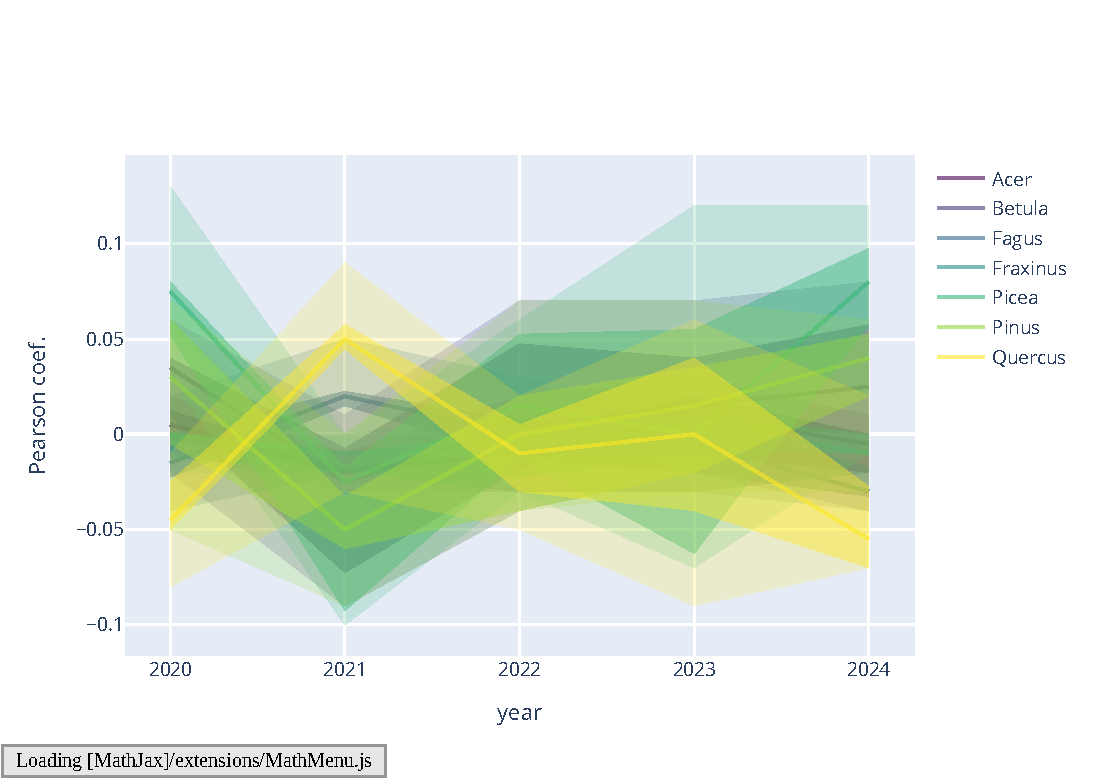
\includegraphics[width=0.9\linewidth, trim={10pt 20pt 10pt 40pt}, clip]{figures/figures_climate/genus_corr.pdf}
    \caption{Median and quantiles of Pearson correlations between changes in tree genera maps predicted by classification and differences in meteorological conditions.}
    \label{fig:genus_corr}
\end{figure}

The representative medians of the variables shown in Fig.\,\ref{fig:selected_variables_stats} were calculated for the years 2010 to 2017. The differences between these medians and those for each individual year from 2020 to 2024 were analyzed and correlated with the discrepancies between classification predictions and actual values. These results are summarized in Fig.\,\ref{fig:genus_corr}. This figure suggests that, over a short-term period of 5 years, the 7 most prominent European tree genera were not significantly affected by climate change. However, this does not account for potential long-term impacts, where even small changes could have substantial effects on ecological dynamics. Additionally, the analysis is limited to Europe, which may experience less pronounced climate changes compared to other regions that are more severely affected. Furthermore, the study does not consider less frequent tree genera, which might be more sensitive to climate change and could exhibit different patterns of response.

\begin{figure}[ht]
    \centering
    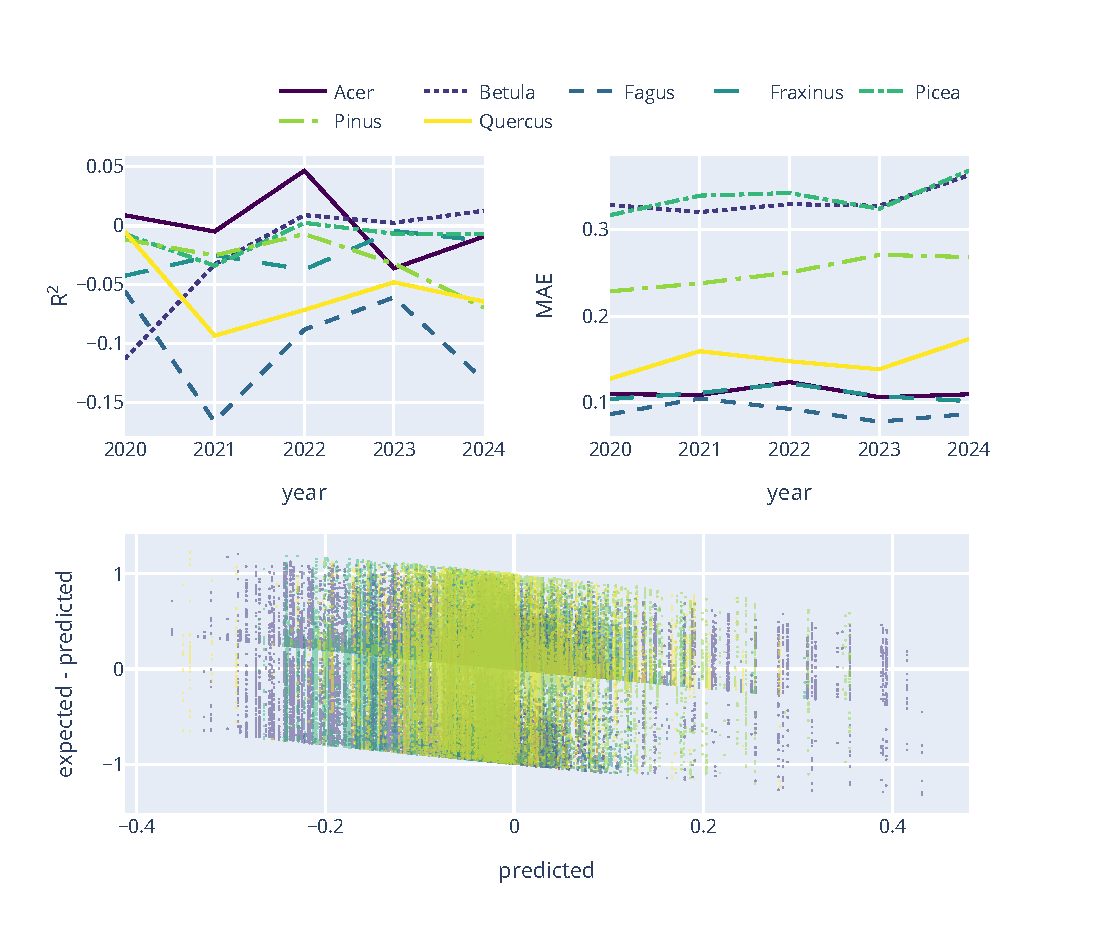
\includegraphics[width=0.9\linewidth, trim={10pt 20pt 10pt 40pt}, clip]{figures/figures_climate/regression_results.pdf}
    \caption{R$^2$ score of a narrow fully-connected regression neural network using meteorological change maps as predictors for genera change maps derived from tree classification.}
    \label{fig:regression_results}
\end{figure}

To further verify the results shown in Fig.\,\ref{fig:genus_corr}, a narrow fully-connected regression neural network was developed. This network used the change map of meteorological variables as predictors to estimate changes in the tree genera maps.